\documentclass{beamer}
\setbeamertemplate{navigation symbols}[horizontal]
\usepackage{pgfpages}
\usetheme{d2s}
\usepackage{graphicx}
\usepackage{tcolorbox}
\usepackage[export]{adjustbox}
\usepackage{listings}
\usepackage{xcolor}
\usepackage{booktabs}
\usepackage{amsmath}
\usepackage{upquote}
\usepackage{tikz}
\usetikzlibrary{positioning, arrows.meta, shapes.geometric}

\definecolor{codegreen}{rgb}{0,0.6,0}
\definecolor{numbercolor}{rgb}{0.5,0.5,0.5}
\definecolor{stringcolor}{rgb}{0.58,0,0.82}
\definecolor{backcolour}{rgb}{0.95,0.95,0.92}
\definecolor{highlightblue}{RGB}{30,100,200}
\definecolor{highlightorange}{RGB}{220,100,10}
\definecolor{highlightgreen}{RGB}{20,150,60}

\lstdefinestyle{mystyle}{
    backgroundcolor=\color{backcolour},
    commentstyle=\color{codegreen},
    keywordstyle=\color{magenta},
    numberstyle=\tiny\color{numbercolor},
    stringstyle=\color{stringcolor},
    basicstyle=\ttfamily\footnotesize,
    breakatwhitespace=false,
    breaklines=true,
    captionpos=b,
    keepspaces=true,
    numbers=left,
    numbersep=5pt,
    showspaces=false,
    showstringspaces=false,
    showtabs=false,
    tabsize=2
}
\lstset{style=mystyle}

\newcommand{\monthyeardate}{\ifcase \month \or January\or February\or March\or %
April\or May \or June\or July\or August\or September\or October\or November\or %
December\fi, \number \year}

%%%%%%%%%%%%%%%%%%%%%%%%%%%%%%%
% Information for Title Slide %
%%%%%%%%%%%%%%%%%%%%%%%%%%%%%%%

\title[]{Agentic AI Bootcamp}
\subtitle[]{Controlling LLM Output: Inference Parameters}
\author[]{MAJ Sean Coffey}
\institute{Army Cyber Institute, U.S. Military Academy}
\date{\monthyeardate}

\begin{document}

%%%%%%%%%%%%%%%%%%%%%
% Title Slide       %
%%%%%%%%%%%%%%%%%%%%%
{\DivisionLogo
\begin{frame}[plain,noframenumbering]
    \titlepage
    \note{This module builds directly on the LLM Fundamentals content. We now go deeper into the
    parameters that allow us to precisely control how an LLM generates text --- critical knowledge
    for building reliable agentic systems.}
\end{frame}
}

% --- Learning Objectives ---
\begin{frame}{Learning Objectives}
    By the end of this module, you will be able to:
    \begin{itemize}
        \item \textbf{Explain} how LLMs produce token probability distributions and why that matters.
        \item \textbf{Configure} Temperature, Top-K, and Top-P to tune output creativity vs.\ determinism.
        \item \textbf{Apply} Frequency and Presence Penalties to reduce repetition.
        \item \textbf{Use} Stop Sequences to control output boundaries in agent pipelines.
        \item \textbf{Select} the right parameter combination for a given task (code, creative, structured output).
    \end{itemize}
\end{frame}

% -----------------------------------------------
\section{How LLMs Generate Text}
% -----------------------------------------------

\begin{frame}{Step Zero: What is the Model Actually Doing?}
    \begin{block}{Next-Token Prediction}
        At each step the model produces a \textbf{probability distribution} over its entire vocabulary
        (30K--130K+ tokens). A \emph{sampling strategy} then selects the next token from that distribution.
    \end{block}
    \vspace{0.3cm}
    \begin{enumerate}
        \item Input tokens are encoded and passed through the Transformer.
        \item The final hidden state is projected through an \emph{LM Head} (linear layer) to produce
              \textbf{logits} --- one real-valued score per vocabulary token.
        \item Logits are converted to probabilities via \textbf{softmax}:
              \[
                  P(w_i) = \frac{e^{z_i}}{\sum_j e^{z_j}}
              \]
        \item Parameters below \emph{modify the logits or the sampling procedure} before the token is drawn.
    \end{enumerate}
    \note{Think of logits as raw scores. The softmax squashes them into a valid probability distribution.
    Everything we discuss today happens between step 2 and step 4.}
\end{frame}

\begin{frame}{The Probability Distribution --- A Toy Example}
    \centering
    \small
    After the prompt \texttt{"The capital of France is"}, the model's top-5 logits might be:

    \vspace{0.3cm}
    \begin{tabular}{@{}lrr@{}}
        \toprule
        \textbf{Token} & \textbf{Logit} & \textbf{Prob (\%)} \\ \midrule
        \texttt{Paris}     & 14.2 & 68.3 \\
        \texttt{Lyon}      &  9.8 &  3.4 \\
        \texttt{Marseille} &  9.1 &  2.5 \\
        \texttt{Nice}      &  8.7 &  1.7 \\
        \texttt{the}       &  7.2 &  0.8 \\
        \textit{(other 50K+ tokens)} & $\cdots$ & 23.3 \\ \bottomrule
    \end{tabular}

    \vspace{0.4cm}
    \begin{alertblock}{Key Insight}
        \textbf{Greedy decoding} always picks \texttt{Paris} (highest probability).
        \textbf{Sampling} may occasionally pick \texttt{Lyon} --- which is sometimes desirable.
    \end{alertblock}
\end{frame}

% -----------------------------------------------
\section{Temperature}
% -----------------------------------------------

\begin{frame}{Temperature: The Creativity Dial}
    \begin{block}{Definition}
        Temperature $T$ is applied to the logits \emph{before} softmax:
        \[
            P(w_i) = \frac{e^{z_i / T}}{\sum_j e^{z_j / T}}
        \]
    \end{block}

    \vspace{0.2cm}
    \begin{columns}
        \column{0.48\textwidth}
        \textbf{Low Temperature ($T < 1$):}
        \begin{itemize}
            \item Divides logits by a small number, \emph{sharpening} the distribution.
            \item Model strongly prefers the highest-probability token.
            \item $T \to 0$: effectively greedy decoding.
        \end{itemize}

        \column{0.48\textwidth}
        \textbf{High Temperature ($T > 1$):}
        \begin{itemize}
            \item Divides logits by a large number, \emph{flattening} the distribution.
            \item Model spreads probability mass more evenly.
            \item $T \to \infty$: uniform random selection.
        \end{itemize}
    \end{columns}
\end{frame}

\begin{frame}{Temperature: Effect on the Distribution}
    \centering
    \small
    Prompt: \texttt{"The soldier's mission was to"} --- effect of $T$ on top-5 tokens:

    \vspace{0.2cm}
    \begin{tabular}{@{}lccc@{}}
        \toprule
        \textbf{Token} & \textbf{$T=0.3$} & \textbf{$T=1.0$} & \textbf{$T=1.8$} \\ \midrule
        \texttt{secure}    & 91.2\% & 38.5\% & 22.1\% \\
        \texttt{locate}    &  5.3\% & 20.1\% & 16.8\% \\
        \texttt{defend}    &  2.1\% & 15.4\% & 14.5\% \\
        \texttt{identify}  &  1.1\% &  9.2\% & 12.3\% \\
        \texttt{infiltrate}&  0.3\% &  7.8\% & 11.9\% \\ \bottomrule
    \end{tabular}

    \vspace{0.3cm}
    At $T=0.3$: \texttt{secure} wins almost every time (predictable). \\
    At $T=1.8$: all five tokens are plausible candidates (diverse).
    \note{This is a synthetic example to illustrate the math. In your notebook lab you will see real
    GPT-2 output shift with temperature.}
\end{frame}

\begin{frame}{Temperature: Practical Guidance}
    \begin{table}
        \centering
        \small
        \begin{tabular}{@{}lll@{}}
            \toprule
            \textbf{Temperature} & \textbf{Behavior} & \textbf{Best For} \\ \midrule
            $0.0$        & Fully deterministic (greedy)   & Tool calling, SQL generation       \\
            $0.1$--$0.3$ & Near-deterministic             & Code generation, fact lookup       \\
            $0.5$--$0.7$ & Balanced                       & Summarization, Q\&A, agents        \\
            $0.8$--$1.0$ & Moderate creativity            & Conversational assistants          \\
            $1.2$--$1.5$ & High diversity                 & Creative writing, brainstorming    \\
            $\geq 1.8$   & Very random (often incoherent) & Data augmentation, adversarial     \\ \bottomrule
        \end{tabular}
    \end{table}

    \vspace{0.2cm}
    \begin{alertblock}{Agentic AI Rule of Thumb}
        Set $T = 0.0$ to $0.2$ when the agent is \textbf{calling tools or producing structured output}.
        Use $T = 0.5$--$0.8$ for \textbf{reasoning and planning} steps.
    \end{alertblock}
\end{frame}

% -----------------------------------------------
\section{Sampling Strategies}
% -----------------------------------------------

\begin{frame}{Top-K Sampling}
    \begin{block}{Definition}
        After computing probabilities, \textbf{keep only the $K$ highest-probability tokens}
        and redistribute the probability mass among them.
    \end{block}

    \vspace{0.2cm}
    \begin{columns}
        \column{0.55\textwidth}
        \textbf{Example ($K = 3$):}
        \begin{enumerate}
            \item Compute full distribution over 50K tokens.
            \item Zero out all tokens except the top 3.
            \item Re-normalize to sum to 1.
            \item Sample from those 3 candidates.
        \end{enumerate}

        \column{0.42\textwidth}
        \textbf{Trade-offs:}
        \begin{itemize}
            \item Prevents selection of very low-probability (incoherent) tokens.
            \item Fixed $K$ can be too large (flat distribution) or too small (misses valid alternatives) depending on context.
            \item Commonly set between $K = 20$ and $K = 100$.
        \end{itemize}
    \end{columns}
\end{frame}

\begin{frame}{Top-P (Nucleus) Sampling}
    \begin{block}{Definition}
        Instead of a fixed count, keep the \textbf{smallest set of tokens whose cumulative
        probability exceeds $p$}, then sample from that set.
    \end{block}

    \vspace{0.2cm}
    \begin{columns}
        \column{0.55\textwidth}
        \textbf{Example ($p = 0.90$):}
        \begin{enumerate}
            \item Sort tokens by probability (descending).
            \item Add tokens to the ``nucleus'' until cumulative $\geq 0.90$.
            \item Renormalize and sample.
        \end{enumerate}

        \column{0.42\textwidth}
        \textbf{Why it's adaptive:}
        \begin{itemize}
            \item When the model is \emph{confident}, the nucleus is small (few tokens cover 90\%).
            \item When the model is \emph{uncertain}, the nucleus is large (many tokens contribute).
            \item Adapts dynamically --- Top-K cannot do this.
        \end{itemize}
    \end{columns}

    \vspace{0.1cm}
    \begin{alertblock}{}
        Top-P is generally preferred over Top-K in modern LLM deployments.
        Common value: $p = 0.95$.
    \end{alertblock}
\end{frame}

\begin{frame}{Top-K vs.\ Top-P: A Comparison}
    \centering
    \small
    \begin{tabular}{@{}lll@{}}
        \toprule
        \textbf{Property} & \textbf{Top-K} & \textbf{Top-P (Nucleus)} \\ \midrule
        Selection basis     & Fixed count                & Cumulative probability       \\
        Adapts to confidence & No                        & Yes                          \\
        Risk (confident dist.) & May include junk tokens  & Nucleus is small/safe        \\
        Risk (flat dist.)      & Misses valid tokens      & Nucleus expands automatically \\
        Typical value       & $K = 40$--$100$            & $p = 0.90$--$0.95$           \\
        Can be combined?    & Yes --- apply K first, then P & Yes --- order matters    \\ \bottomrule
    \end{tabular}

    \vspace{0.3cm}
    \textbf{Common production config:} Temperature $T=0.7$ + Top-P $p=0.95$ (no Top-K).
\end{frame}

\begin{frame}{Combining Temperature, Top-K, and Top-P}
    The parameters are applied \textbf{in sequence}:

    \vspace{0.3cm}
    \centering
    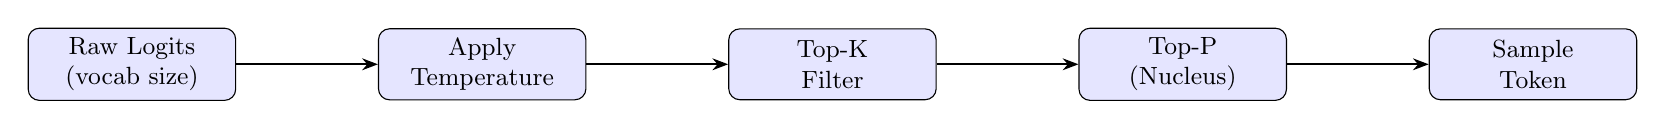
\begin{tikzpicture}[node distance=1.8cm, auto,
        box/.style={rectangle, draw, rounded corners, fill=blue!10,
                    text width=2.4cm, align=center, minimum height=0.9cm, font=\small},
        arrow/.style={-{Stealth[length=2mm]}, thick}]

        \node[box] (logits)  {Raw Logits\\(vocab size)};
        \node[box, right=of logits] (temp)   {Apply\\Temperature};
        \node[box, right=of temp]   (topk)   {Top-K\\Filter};
        \node[box, right=of topk]   (topp)   {Top-P\\(Nucleus)};
        \node[box, right=of topp]   (sample) {Sample\\Token};

        \draw[arrow] (logits)  -- (temp);
        \draw[arrow] (temp)    -- (topk);
        \draw[arrow] (topk)    -- (topp);
        \draw[arrow] (topp)    -- (sample);
    \end{tikzpicture}

    \vspace{0.4cm}
    \begin{itemize}
        \item Temperature reshapes the full distribution first.
        \item Top-K prunes to the $K$ highest after temperature is applied.
        \item Top-P further prunes to the cumulative nucleus.
        \item Sampling draws one token from the remaining set.
    \end{itemize}
\end{frame}

% -----------------------------------------------
\section{Penalty Parameters}
% -----------------------------------------------

\begin{frame}{Frequency \& Presence Penalties}
    Both penalties \textbf{reduce repetition} but operate differently:

    \vspace{0.2cm}
    \begin{block}{Frequency Penalty ($\alpha_f$, typically 0.0--2.0)}
        Subtracts from a token's logit proportionally to \emph{how many times it has appeared} in the
        current output:
        \[
            z'_i = z_i - \alpha_f \cdot \text{count}(i)
        \]
        The more a word has been used, the harder it is to use again.
    \end{block}

    \begin{block}{Presence Penalty ($\alpha_p$, typically 0.0--2.0)}
        A \emph{flat} penalty applied once a token has appeared at least once:
        \[
            z'_i = z_i - \alpha_p \cdot \mathbb{1}[\text{count}(i) > 0]
        \]
        Discourages any repetition of already-seen tokens, regardless of frequency.
    \end{block}
\end{frame}

\begin{frame}{When to Use Repetition Penalties}
    \begin{table}
        \centering
        \small
        \begin{tabular}{@{}lll@{}}
            \toprule
            \textbf{Penalty} & \textbf{Good For} & \textbf{Risk} \\ \midrule
            Frequency (low, 0.1--0.5) & Long-form text, reports       & Minimal --- safe default   \\
            Frequency (high, $>$1.0)  & Extreme diversity             & May force unnatural wording \\
            Presence (low, 0.1--0.3)  & Conversations, story variety  & Fine for most tasks         \\
            Presence (high, $>$1.0)   & Preventing topic re-mention   & Hurts factual tasks (must repeat nouns!) \\
            None (0.0)                & Factual Q\&A, code, structured output & Repetitive loops in long outputs \\ \bottomrule
        \end{tabular}
    \end{table}

    \begin{alertblock}{Agentic AI Warning}
        High presence penalties can cause agents to \textbf{avoid re-mentioning key entities}
        (e.g., a file path or variable name) that must be repeated correctly.
        Use low values ($\leq 0.3$) in agent pipelines or set to 0.
    \end{alertblock}
\end{frame}

% -----------------------------------------------
\section{Stop Sequences \& Max Tokens}
% -----------------------------------------------

\begin{frame}{Stop Sequences}
    \begin{block}{Definition}
        A stop sequence is a \textbf{string (or list of strings)} that, when generated by the model,
        causes generation to immediately halt.
    \end{block}

    \vspace{0.2cm}
    \textbf{Why they matter in Agentic AI:}
    \begin{itemize}
        \item \textbf{Structured Output:} Halt after a closing \texttt{\}} or \texttt{```} to capture valid JSON/code.
        \item \textbf{Turn Boundaries:} Stop at \texttt{Human:} to prevent the model from simulating the user.
        \item \textbf{Tool-Call Markers:} Stop at \texttt{<tool\_call>} to hand off to the executor.
        \item \textbf{Cost Control:} Prevents the model from generating beyond useful content.
    \end{itemize}

    \vspace{0.2cm}
    \textbf{Examples:}
    \begin{lstlisting}[language=Python]
stop_sequences = ["\nHuman:", "```\n", "</tool_call>", "\n\n---"]
    \end{lstlisting}
    \note{Stop sequences are one of the most underutilized yet powerful tools in agent design.
    They enforce boundaries without needing post-processing heuristics.}
\end{frame}

\begin{frame}{Max Tokens / Max New Tokens}
    \begin{itemize}
        \item \textbf{Max Tokens:} Hard upper limit on the number of tokens the model will generate.
        \item Prevents run-away generation and controls \textbf{cost} (you pay per output token).
        \item Distinct from context window --- max tokens limits the \emph{output}, not the input.
    \end{itemize}

    \vspace{0.3cm}
    \begin{table}
        \centering
        \small
        \begin{tabular}{@{}lll@{}}
            \toprule
            \textbf{Task} & \textbf{Suggested Max Tokens} & \textbf{Notes} \\ \midrule
            Sentiment classification   & 10--20    & ``Positive'' or ``Negative''       \\
            Named entity extraction    & 50--200   & JSON list of entities              \\
            Paragraph summarization    & 100--300  & One to three sentences             \\
            Code generation (function) & 300--800  & Stop at \texttt{```} too           \\
            Long-form report           & 2000+     & Use streaming; watch cost          \\
            Agent reasoning step       & 500--1500 & Balance depth vs.\ latency         \\ \bottomrule
        \end{tabular}
    \end{table}
\end{frame}

% -----------------------------------------------
\section{Structured Output \& Logit Biasing}
% -----------------------------------------------

\begin{frame}{Logit Bias: Forcing or Forbidding Tokens}
    \begin{block}{Definition}
        A dictionary mapping token IDs to a bias value added to their logit before sampling.
        Range: typically $-100$ (effectively ban) to $+100$ (virtually guarantee).
    \end{block}

    \vspace{0.2cm}
    \textbf{Use cases:}
    \begin{itemize}
        \item \textbf{Classification tasks:} Force output to be one of \texttt{\{A, B, C, D\}} by
              biasing only those tokens to $+100$ and everything else to $-100$.
        \item \textbf{Safety:} Permanently suppress known harmful tokens.
        \item \textbf{Structured output:} Constrain JSON keys to a fixed schema
              (grammar-constrained decoding is a more advanced version of this).
    \end{itemize}

    \begin{alertblock}{Modern Alternative}
        Many APIs now offer \textbf{JSON Mode} or \textbf{Structured Outputs} (OpenAI, Anthropic, Gemini),
        which handle logit biasing internally to guarantee valid schema-conforming output.
    \end{alertblock}
\end{frame}

% -----------------------------------------------
\section{Complete Parameter Reference}
% -----------------------------------------------

\begin{frame}{The Complete Parameter Cheat Sheet}
    \centering
    \tiny
    \begin{tabular}{@{}llll@{}}
        \toprule
        \textbf{Parameter}     & \textbf{Range}    & \textbf{Default} & \textbf{Effect} \\ \midrule
        Temperature            & 0.0 -- 2.0        & 1.0              & Controls randomness \\
        Top-K                  & 1 -- vocab size   & Off              & Limits candidate pool to K tokens \\
        Top-P                  & 0.0 -- 1.0        & 1.0 (off)        & Nucleus sampling by cumulative prob \\
        Frequency Penalty      & 0.0 -- 2.0        & 0.0              & Penalizes tokens by usage count \\
        Presence Penalty       & 0.0 -- 2.0        & 0.0              & Penalizes any previously used token \\
        Stop Sequences         & List of strings   & None             & Halts generation at a specific string \\
        Max New Tokens         & 1 -- ctx limit    & Model default    & Maximum output length \\
        Logit Bias             & Token$\to$float   & None             & Boosts or suppresses specific tokens \\
        Seed                   & Integer           & Random           & Reproducible sampling at $T>0$ \\ \bottomrule
    \end{tabular}

    \vspace{0.3cm}
    \normalsize
    \begin{block}{Recommended Configurations}
        \textbf{Agent tool-calling:} $T=0.0$, stop=\texttt{["\textless/tool\_call\textgreater"]} \\
        \textbf{Creative writing:} $T=1.2$, Top-P=0.95, Freq=0.3 \\
        \textbf{Factual Q\&A:} $T=0.2$, Top-P=0.9, no penalties \\
        \textbf{Code generation:} $T=0.1$, stop=\texttt{["```"]}
    \end{block}
\end{frame}

\begin{frame}{Parameter Interactions: Common Pitfalls}
    \begin{itemize}
        \item \textbf{Temperature 0 + Top-P 0.9:} Top-P is irrelevant --- $T=0$ makes sampling
              deterministic before Top-P is applied. Use one or the other.
        \item \textbf{High Frequency Penalty + Factual Tasks:} The model may paraphrase proper nouns
              it should repeat verbatim (e.g., names, code identifiers).
        \item \textbf{Low Max Tokens + Complex Reasoning:} Truncates the chain-of-thought, often
              producing a worse final answer or a cut-off JSON blob.
        \item \textbf{No Stop Sequences in Multi-Turn:} Model may continue generating dialogue for
              imaginary users, inflating cost and breaking agent state machines.
        \item \textbf{High Temperature + Structured Output:} Random sampling breaks JSON schema
              compliance. Always use $T \leq 0.3$ (or JSON mode) for structured tasks.
    \end{itemize}
\end{frame}

% -----------------------------------------------
\section{Summary}
% -----------------------------------------------
\begin{frame}{Summary}
    \begin{itemize}
        \item LLMs produce a \textbf{logit distribution} over every token at each step.
              Parameters modify how the model samples from that distribution.
        \item \textbf{Temperature} reshapes the distribution:
              low $\Rightarrow$ deterministic, high $\Rightarrow$ creative.
        \item \textbf{Top-K} prunes to a fixed candidate count;
              \textbf{Top-P} prunes adaptively based on cumulative probability.
        \item \textbf{Frequency \& Presence Penalties} reduce repetition with different mechanics.
        \item \textbf{Stop Sequences} are essential for agentic pipelines to enforce output boundaries.
        \item No single configuration is universal --- \textbf{match parameters to the task}.
    \end{itemize}

    \vspace{0.2cm}
    \textbf{Up next:} Prompt Engineering --- controlling the model through input, not just sampling.
\end{frame}

\end{document}
